\chapter{Results}\label{chap:res}
\gls{sys} is able to produce biologically relevant dimensionality reductions that allow us to make better reduce models for \gls{cfps} systems.
This chapter demonstrates the following:
\begin{itemize}
\item \gls{pca} and naive \glspl{vae} cannot learn good representations of different models, while a Corr-VAE can.
\item The separation between the different models improves as the number of latent dimensions increases.
This is replicated across different \gls{cfps} systems.
\item As noise is added to the input dataset, Corr-VAE performance falls off, showing that it is learning real trends.
\item A Corr-VAE can be used to reduce \glspl{gem} to create \gls{cfps} models that correlate better with experimental data.
\end{itemize}

\section{Can a \gls{vae} distinguish between fluxes generated from different experimental conditions?}
I first investigated whether or not a \gls{vae} can learn how changes in the experimental conditions affect the underlying \gls{cfps} system.
To be useful for extracting information about the underlying cell-free system, a \gls{vae} would need to be able to distinguish between different starting experimental conditions.
In order to assess how well a \gls{vae} is learning the differences between experimental conditions, I examined its latent space.
If the \gls{vae} performs well, we should see a clear separation between fluxes generated from different experimental conditions.
This set of experiments was run on the set of fluxes generated from our manual dataset.
The \gls{pca} and regular \gls{vae} are trained on the flat version of the manual dataset, while our Corr-VAE is trained on the stacked version.
All three techniques then project the same test dataset into 2 dimensions for visualization purposes.
The \gls{vae} and the Corr-VAE have identical network structures as described in Section \ref{sec:vae}.

Figure \ref{fig:vae_pca} shows the latent space of a basic \gls{vae} as well as the first two principal components of the \gls{pca}.
Both dimensionality reduction techniques fail to uncover the underlying structure of the fluxes.
This demonstrates that naive applications of a \gls{vae} or \gls{pca} cannot learn the differences between the various starting experimental conditions.

\begin{figure}[t!]
\begin{center}
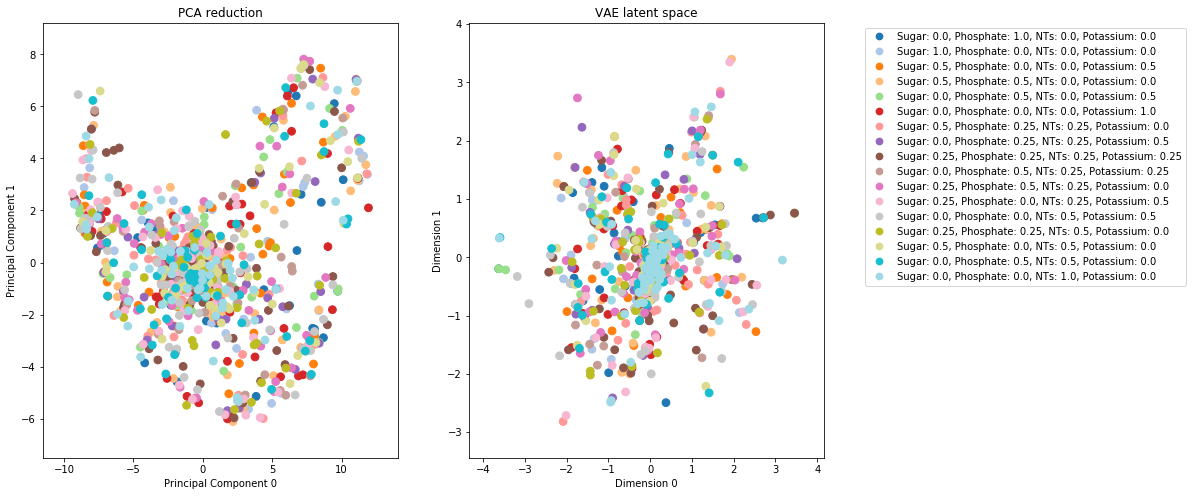
\includegraphics[width=1.2\textwidth]{figs/vae_vs_pca_latent.png}
\caption[Comparison of the latent dimensions \gls{pca} and \gls{vae}]{Left: first two principal components of a \gls{pca} on our test dataset.
Right: the two latent dimensions of a trained \gls{vae} with the classic loss function.
Different colors represent different experimental conditions.
Neither \gls{pca} nor a basic \gls{vae} can learn a clear representation of the different models we are using.}
\label{fig:vae_pca}
\end{center}
\end{figure}

However, a Corr-VAE is able to recover clear distinctions between the different experimental conditions.
Figure \ref{fig:corrvae_2d} plots the latent space of our Corr-VAE.
Whereas the experimental conditions cannot be recovered in the latent space of the \gls{vae}, the latent space of the Corr-VAE clearly distinguishes between the different starting conditions.
While \gls{pca} is a popular dimensionality reduction technique in biology, these results suggest that Corr-VAE may be a more effective way to discover relationships in biological data.

\begin{figure}[t!]
\begin{center}
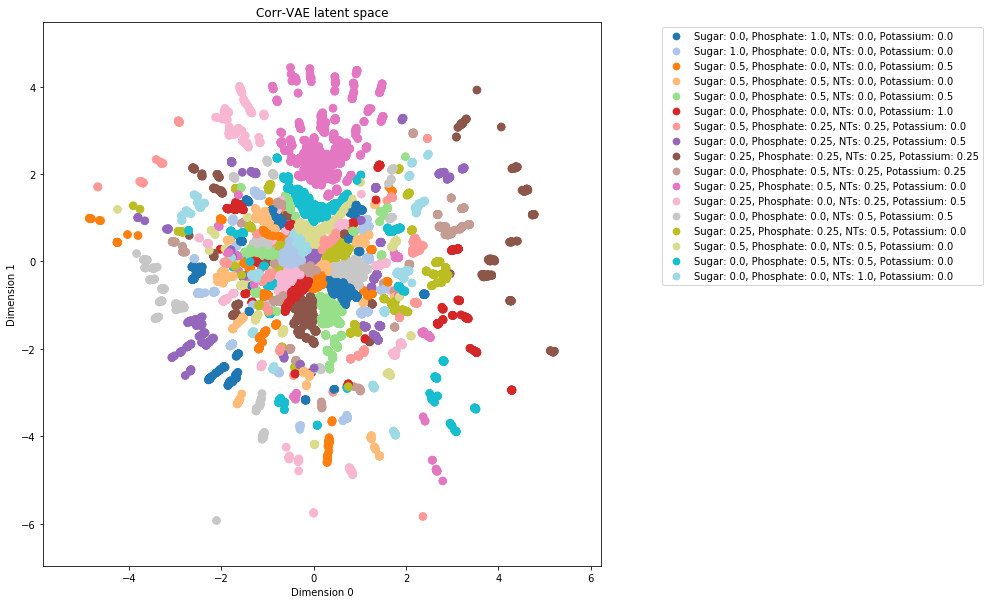
\includegraphics[width=1.01\textwidth]{figs/corrvae_hand_2d_latent.png}
\caption[Latent dimensions of our Corr-VAE network]{Different colors represent different experimental conditons.
This plot shows the two latent dimensions of a trained Corr-VAE.
Colors cluster together and show that a Corr-VAE can recover the original models.}
\label{fig:corrvae_2d}
\end{center}
\end{figure}

The original flux datasets have around 2600 reactions, so using a latent space of only 2 dimensions is a very severe dimensionality reduction.
In addition to the Corr-VAE with latent dimension 2, shown above, I also trained a Corr-VAE with a 10 dimensional latent space.
In order to visualize the latent space of this Corr-VAE, the 10-dimensional latent space was projected down to 2 dimensions using the \gls{tsne} method~\cite{maaten2008visualizing}.
Figure \ref{fig:manual_10d} shows that using a 10-dimensional latent space with a Corr-VAE is also able to clearly separate different starting experimental conditions.
The separation between models is even more clear in this case, and suggests that more latent dimensions allow for richer latent representations of each model.

I also show that this technique can generalize across different \gls{cfps} systems.
Figure \ref{fig:karim_10d} is generated using the same 10-dimensional structure as the Corr-VAE in Figure \ref{fig:manual_10d}, but on the Karim dataset instead of the Manual dataset.

\begin{figure}[t!]
\begin{center}
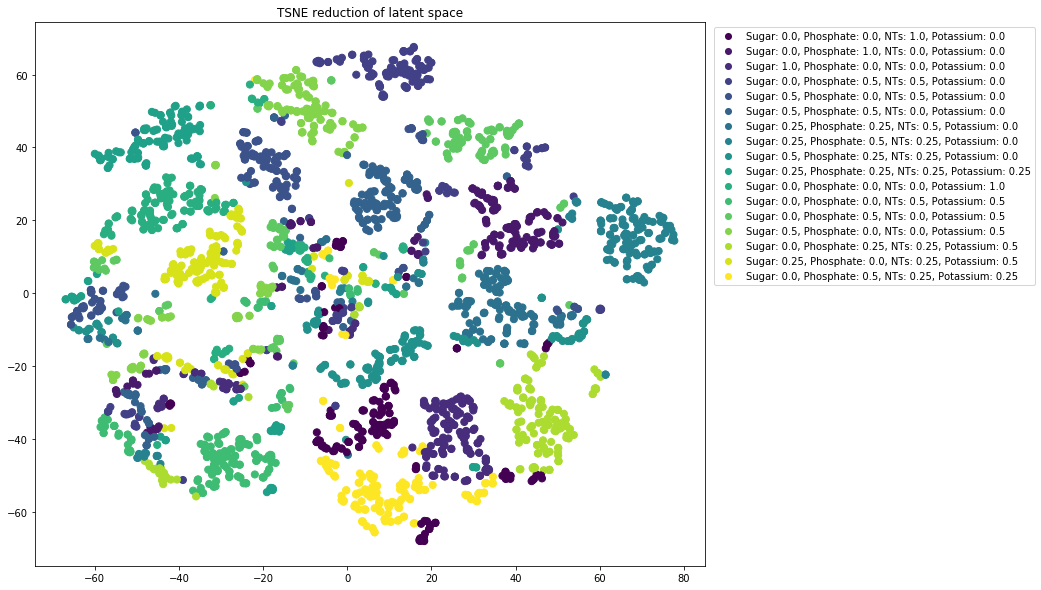
\includegraphics[width=1.01\textwidth]{figs/TSNE_hand_latent10.png}
\caption[Projection of the latent space of a 10-dimensional Corr-VAE trained on the Manual dataset]{Different colors represent different experimental conditons.
This plot shows a \gls{tsne} projection of the 10-dimensional latent space of a Corr-VAE trained on the Manual dataset.
Adding more latent dimensions allows better reconstruction of the invidual models.
}
\label{fig:manual_10d}
\end{center}
\end{figure}

\begin{figure}[t!]
\begin{center}
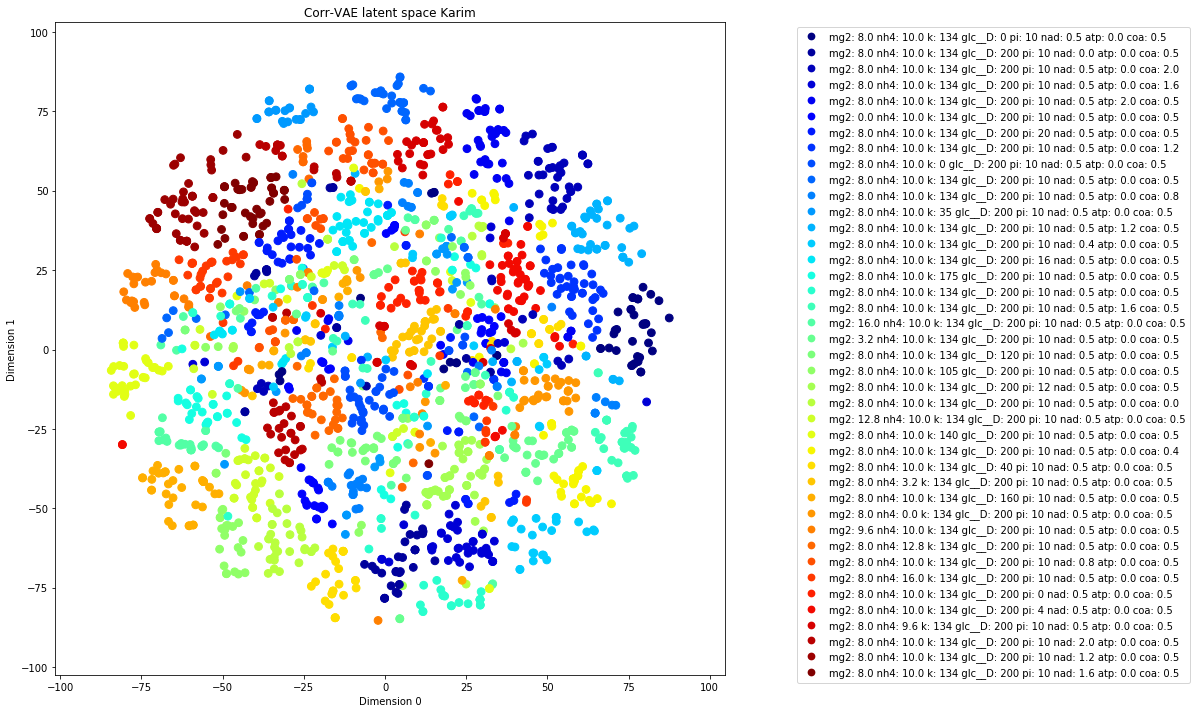
\includegraphics[width=1.01\textwidth]{figs/corrvae_karim_10d_latent.png}
\caption[Projection of the latent space of a 10-dimensional Corr-VAE trained on the Karim dataset]{Different colors represent different experimental conditons.
This plot shows a \gls{tsne} projection of the 10-dimensional latent space of a Corr-VAE trained on the Karim dataset.
Our Corr-VAE is able to reconstruct the individual models for multiple types of \gls{cfps} systems.
}
\label{fig:karim_10d}
\end{center}
\end{figure}

\section{Noise experiments}
In order to validate that the Corr-VAE was performing as intended, I ran a number of experiments to ensure that these results were not due to noise.
Figure \ref{fig:recon_stds} plots the standard deviations of each of the reactions for the test dataset as well as the reconstructed dataset.
The reconstructed dataset maintains a very similar shape to the original dataset, while also reducing the standard deviation of fluxes with each reaction.
This shows that the Corr-VAE is not drastically changing the structure of the fluxes to produce biologically impossible fluxes.
Additionally, this plot implies that the Corr-VAE could also be used to de-noise our dataset.

\begin{figure}[t!]
\begin{center}
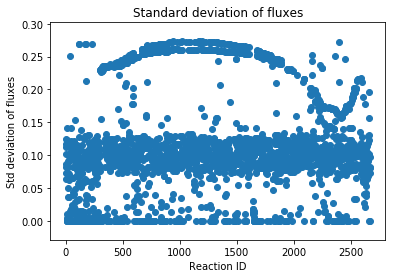
\includegraphics[width=1.01\textwidth]{figs/Reconstructed_stds.png}
\caption[Reconstructing fluxes reduces the amount of noise]{Reconstructed fluxes reduce the amount of noise while also maintaining the shape}
\label{fig:recon_stds}
\end{center}
\end{figure}

Another potential issue was that the Corr-VAE was only learning how to artificially order the objective flux.
Although the correlation error was smaller than the reconstruction error, the Corr-VAE could be generating correlations instead of discovering them, just to reduce its loss function.
To show that this was not the case, I generated a new, biased dataset where the objective fluxes were already highly correlated to our experimental data.
Figure \ref{fig:noise} shows what happens when we add noise to this biased dataset.
The correlation between the starting data and the experimental data is around 0.78 and is shown by the green line.
After running the biased fluxes through a Corr-VAE, the correlation is even higher, as evidenced by the blue line.
But, as noise is added to the data by randomly drawing from a normal distribution and adding it to the flux for each reaction, the correlation begins to fall.
This shows that the Corr-VAE architecutre does not create correlations with random data, but is learning the correlation from the underlying data.

\begin{figure}[t!]
\begin{center}
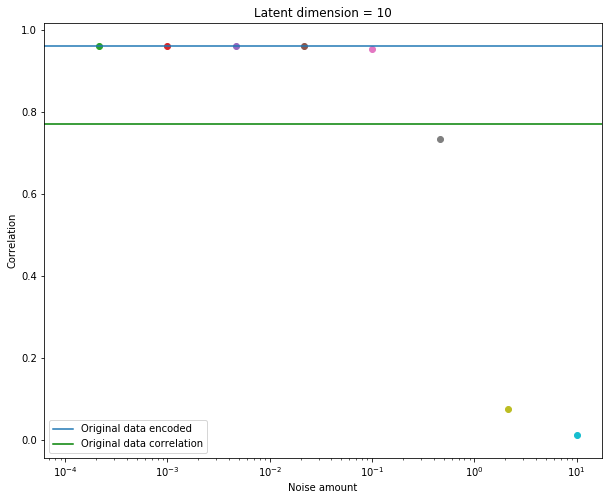
\includegraphics[width=1.01\textwidth]{figs/Noise_add.png}
\caption[Noise added to input data reduces the efficacy of a Corr-VAE]{Adding noise to the data reduces the correlation from our \gls{vae}}
\label{fig:noise}
\end{center}
\end{figure}

\section{Comparison of reduced models}\label{sec:cmp}
A key goal for \gls{sys} was to produce reduced models that could accurately explain experimental data.
I tested this by solving for the optimal flux distribution for each model of our reaction conditions.
A model's ability to explain the experimental data was then assessed using the correlation between the predicted output and the real biological output.
Table \ref{tab:cmp} shows the results for each of our starting models that are at the \gls{gem} scale as well as some reduced models.
As expected, we found that the full-scale \glspl{gem} have very low correlations, between $0.14$ and $0.24$.
This models are intended to describe living \ecoli cells and thus do a poor job of modeling \gls{cfps} systems.

We also compare our model to pre-existing pruned models that other algorithms have created.
For instance, the ColiPruned model from NetworkReducer has a correlation of $0.34$ with our biological data.
This is better than the full-scale genome models, though it is not as good as our customized cell-free models.
This make sense because the goal of NetworkReducer is to reduce to a minimal core model, not to specify it for cell-free systems.
Our system produces models that with more than 2x better correlations than a full-scale \gls{gem}.
While these correlations show that we still cannot perfectly describe the biological system, the reduction is far better than a full-scale model.

\begin{table}[]
\centering
\begin{tabular}{lll}
Dataset        & Uses Corr-VAE? & Correlation \\ \hline
echo\_txtl     & No             & 0.22        \\
echo           & No             & 0.14        \\
manual\_txtl   & No             & 0.23        \\
manual         & No             & 0.24        \\
karim          & No             & 0.17        \\
coli-pruned    & No             & 0.34        \\
echo-reduced   & Yes            & \textbf{0.54}        \\
manual-reduced & Yes            & \textbf{0.50}       \\
karim-reduced  & Yes            & \textbf{0.43}   
\end{tabular}
\caption[Comparison of how well different models correlate with experimental data]{Comparison of how well different models correlate with experimental data.
Models that have been produced by \gls{sys} end in 'reduced'.
Full-scale \glspl{gem} perform the worst, while a reduced model such as the ColiPruned model from NetworkReducer performs slightly better.
Although the reduced models genereated by \gls{sys} cannot fully explain the experimental data, they are able to explain the data better than any other models.
}
\label{tab:cmp}
\end{table}